\section{Binary Features}

Now, assume that \(\mat{X}\) and \(\vec{\beta}\) are fixed and that \(\vec{y} = \mat{X}\vec{\beta} + \vec{\varepsilon}\), where \(\varepsilon_i\) is identically and independently distributed noise with mean zero and finite variance \(\sigma_\varepsilon^2\). We are interested in the expected value of \Cref{eq:orthogonal-solution}. Let \(Z = \tilde{\vec{x}}_j^\T \vec{y} = \tilde{\vec{x}}_j^\T(\mat{X}\vec{\beta} + \vec{\varepsilon})\) and \(d_j = s_j\left(\tilde{\vec{x}}_j^\T \tilde{\vec{x}}_j + \lambda_2\right)\) so that \(\hat{\beta}_j = \st_{\lambda_1}(Z)/d_j\). We start by focusing on the numerator, since the denominator, \(d_j\), is fixed. First observe that
\[
  \E Z = \mu = \E \left( \tilde{\vec{x}}_j^\T (\vec{x}_j\beta_j + \vec{\varepsilon}) \right)  = \tilde{\vec{x}}_j^\T\vec{x}_j \beta_j.
\]
And for the variance, we have
\[
  \var Z = \sigma^2 = \var\left(\tilde{\vec{x}}_j ^\T \vec{\varepsilon}\right) = \sigma_\varepsilon^2 \lVert \tilde{\vec{x}}_j\rVert_2^2 .
\]

The expected value of the soft-thresholding estimator is
\begin{align}
  \label{eq:st-expected-value}
  \E \st_\lambda(Z) & = \int_{-\infty}^\infty \st_\lambda(z) f_Z(z) \du z                                                   \nonumber \\
                    & = \int_{-\infty}^\infty \ind{|z| > \lambda} (z -\sign(z)\lambda) f_Z(z) \du z                         \nonumber \\
                    & = \int_{-\infty}^{-\lambda}(z + \lambda)f_Z(z) \du z + \int_{\lambda}^\infty (z - \lambda)f_Z(z) \du z.
\end{align}
And then the bias of \(\hat\beta_j\) with respect to the true coefficient \(\beta_j^*\) is
\begin{equation}
  \label{eq:betahat-bias}
  \E \hat\beta_j - \beta_j^* = \frac{1}{d_j}\E \st_\lambda(Z) - \beta^*_j.
\end{equation}

Finally, we note that the variance of the soft-thresholding estimator is
\begin{equation}
  \label{eq:st-variance}
  \var {S_\lambda(Z)} = \int_{-\infty}^{-\lambda}(z + \lambda)^2f_Z(z) \du z + \int_{\lambda}^\infty (z - \lambda)^2 f_Z(z) \du z - \left(\E \st_\lambda(Z)\right)^2
\end{equation}
and that the variance of the elastic net estimator is therefore
\begin{equation}
  \label{eq:betahat-variance}
  \var \hat\beta_j = \frac{1}{d_j^2} \var \st_\lambda(Z).
\end{equation}

% \subsection{Normally Distributed Noise}

Next, we add the additional assumption that \(\vec{\varepsilon}\) is normally distributed. Then
\[
  Z \sim \normal\left(\tilde{\vec{x}}_j^\T\vec{x}_j \beta_j, \sigma_\varepsilon^2 \lVert \tilde{\vec{x}}_j\rVert_2^2 \right).
\]
Let \(\theta = -\mu -\lambda_1 \) and \(\gamma = \mu - \lambda_1\). Then the expected value of soft-thresholding of \(Z\) is
\begin{align}
  \E \st_{\lambda_1}(Z) & = \int_{-\infty}^\frac{\theta}{\sigma} (\sigma u - \theta) \pdf(u) \du u + \int_{-\frac{\gamma}{\sigma}}^\infty (\sigma u + \gamma) \pdf(u) \du u                                               \nonumber                      \\
                        & = -\theta \cdf\left(\frac{\theta}{\sigma}\right) - \sigma \pdf\left(\frac{\theta}{\sigma}\right) + \gamma \cdf\left(\frac{\gamma}{\sigma}\right) + \sigma \pdf\left(\frac{\gamma}{\sigma}\right) \label{eq:mean-centered-eval}
\end{align}
where \(\pdf(u)\) and \(\cdf(u)\) are the probability density and cumulative distribution functions of the standard normal distribution, respectively.

Next, we consider what the variance of the elastic net estimator looks like.
Starting with the first term on the left-hand side of \Cref{eq:st-variance}, we have
\begin{align}
  \label{eq:mc-var-part1}
  \int_{-\infty}^{-\lambda_1}(z+ \lambda_1)^2 f_Z(z) \du z & = \sigma^2 \int_{-\infty}^{\frac{\theta}{\sigma}} y^2 \pdf(y) \du y + 2 \theta \sigma \int_{-\infty}^{\frac{\theta}{\sigma}} y \pdf(y) \du y + \theta^2 \int_{-\infty}^{\frac{\theta}{\sigma}} \pdf(y) \du y                                                                                 \\
                                                           & = \frac{\sigma^2}{2} \left( \erf\left(\frac{\theta}{\sigma\sqrt{2}}\right) - \frac{\theta}{\sigma}\sqrt{\frac{2}{\pi}} \exp\left(-\frac{\theta^2}{2\sigma^2}\right) + 1 \right) + 2 \theta \sigma \pdf \left(\frac{\theta}{\sigma}\right) + \theta^2 \cdf\left(\frac{\theta}{\sigma}\right).
\end{align}
Similar computations for the second term on the left-hand side of \Cref{eq:st-variance} yield
\begin{equation}
  \label{eq:mc-var-part2}
  \int_{\lambda_1}^{\infty}(z - \lambda_1)^2 f_Z(z) \du z = \frac{\sigma^2}{2} \left( \erf\left(\frac{\gamma}{\sigma\sqrt{2}}\right) - \frac{\gamma}{\sigma}\sqrt{\frac{2}{\pi}} \exp\left(-\frac{\gamma^2}{2\sigma^2}\right) + 1 \right) + 2 \gamma \sigma \pdf \left(\frac{\gamma}{\sigma}\right) + \gamma^2 \cdf\left(\frac{\gamma}{\sigma}\right).
\end{equation}
Plugging \Cref{eq:mean-centered-eval,eq:mc-var-part1,eq:mc-var-part2} into \Cref{eq:betahat-variance} yields the variance of the estimator. Consequently, we can also compute the mean-squared error via the bias-variance decomposition
\begin{equation}
  \label{eq:betahat-mse}
  \mse (\hat\beta_j, \beta^*_j) = \var\hat\beta_j + \left(\E \hat\beta_j - \beta^*_j\right)^2.
\end{equation}

% \subsubsection{Binary Features}

Our results have so far covered the general case where we have made no assumptions on \(\mat{X}\), except for being non-random. But our main focus in this paper
is the case when \(\vec{x_j}\) is a binary feature with class balance \(q\), that is, \(x_{ij} \in \{0, 1\}\) for all \(i\) and \(\sum_{i=1}^n x_{ij} = nq\).
In this case, we observe that
\[
  \begin{aligned}
    \tilde{\vec{x}}_j^\T \tilde{\vec{x}}_j & = \frac{1}{s_j^2}(\vec{x}_j - \ones c_j)^\T (\vec{x}_j - \ones c_j) = \frac{1}{s^2_j}(nq - 2nq^2 + nq^2) = \frac{nq(1-q)}{s^2_j}, \\
    \tilde{\vec{x}}_j^\T \vec{x}_j         & = \frac{1}{s_j}(\vec{x}_j^\T \vec{x}_j - \vec{x}_j^\T \ones c_j) = \frac{nq(1 - q)}{s_j}.
  \end{aligned}
\]
And consequently
\[
  \mu = \frac{\beta^*_j nq(1 - q)}{s_j}, \qquad \sigma^2 = \frac{\sigma_\varepsilon^2nq(1 - q)}{s^2_j}, \qquad d_j = \frac{nq(1 -q)}{s_j}  + \lambda_2 s_j.
\]
We will allow ourselves to abuse notation and overload the definitions of \(\mu\), \(\sigma^2\), and \(d_j\) as functions of \(q\). Then, an expression for the expected value of the elastic net estimate with respect to \(q\) can be obtained by plugging in \(\mu\) and \(\sigma\) into \Cref{eq:mean-centered-eval}.

We are mainly interested in examining the case when \(\vec{x}_j\) is imbalanced and what effect various approaches to normalizing the features
has on the elastic net estimator. In order to study this, we will parameterize the scaling factors \(s_j\) for \(j  \in [p]\) by \(s_j = (q - q^2)^\delta\), \(\delta \geq 0\).
This includes the cases that we are primary interested in, that is,
\begin{itemize}
  \item \(\delta = 0\): no scaling, which includes min--max and max--abs normalization,
  \item \(\delta = 1/2\): standardization, and
  \item \(\delta = 1\): scaling by the variance.
\end{itemize}
Note that the last of these cases does not correspond to a standard type of normalization. But as we will see, it has some interesting properties in the case of binary features.

A natual consequence of the normal distribution of \(Z\) is that the probability of selection in the elastic net problem is given by
\begin{align*}
  \Pr\left(\hat{\beta}_j \neq 0\right) & = \Pr\left(\st_{\lambda_1}(Z) \neq 0\right)                                                                                         \\
                                       & = \Pr\left(Z > \lambda_1\right) + \Pr\left(Z < -\lambda_1\right)                                                                    \\
                                       & = \cdf\left(\frac{\mu - \lambda_1}{\sigma}\right) + \cdf\left(\frac{- \mu -\lambda_1}{\sigma}\right).                               \\
                                       & = \cdf \left( \frac{\beta_j^*n (q-q^2)^{1/2} - \lambda_1(q-q^2)^{\delta - 1/2}}{\sigma_\varepsilon \sqrt{n}}\right)                 \\
                                       & \phantom{={}} + \cdf \left( \frac{-\beta_j^*n (q-q^2)^{1/2} - \lambda_1(q-q^2)^{\delta - 1/2}}{\sigma_\varepsilon \sqrt{n}}\right).
\end{align*}

Letting \(\theta = -\mu - \lambda_1 \) and \(\gamma = \mu - \lambda_1\), we can express the probability of selection in the limit as \(q \rightarrow 1^+\) as
\[
  \lim_{q \rightarrow 1^+} \Pr(\hat{\beta}_j \neq 0) =
  \begin{cases}
    0                                                                & \text{if } 0 \leq \delta < \frac{1}{2}, \\
    2\cdf\left(-\frac{\lambda_1}{\sigma_\varepsilon \sqrt{n}}\right) & \text{if } \delta = \frac{1}{2},        \\
    1                                                                & \text{if } \delta > \frac{1}{2}.
  \end{cases}
\]

\begin{figure}[htpb]
  \centering
  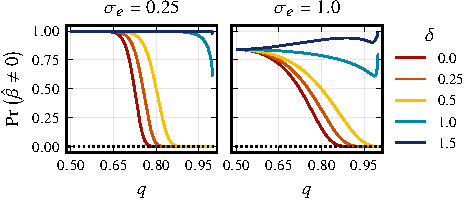
\includegraphics[]{plots/selection_probability.pdf}
  \caption{%
    Probability of selection in the elastic net problem given a measurement noise level \(\sigma_\varepsilon\), a regularization parameter \(\lambda_1\), and a class balance \(q\). The scaling factor is parameterized by \(s_j = (q - q^2)^\delta\), \(\delta \geq 0\). The dotted line represents the asymptotic limit for the standardization case, \(\delta = 1/2\). }
  \label{fig:selection-probability}
\end{figure}

In \Cref{thm:classbalance-bias}, we show what the
bias is under mean-centering and scaling with \(s_j = (q - q^2)^\delta\), \(\delta \geq 0\).

\begin{theorem}
  \label{thm:classbalance-bias}
  If \(\vec{x}_j\) is a binary feature with class balance \(q \in (0, 1)\), \(\lambda_1 \in (0,\infty)\), \(\lambda_2 \in [0,\infty)\), \(\sigma_\varepsilon > 0\), and \(s_j = (q - q^2)^{\delta}\), \(\delta \geq 0\)  then
  \[
    \lim_{q \rightarrow 1^+} \E \hat{\beta}_j =
    \begin{cases}
      0                                                                                                  & \text{if } 0 \leq \delta < \frac{1}{2}, \\
      \frac{2n \beta_j^*}{n + \lambda_2} \cdf\left(-\frac{\lambda_1}{\sigma_\varepsilon \sqrt{n}}\right) & \text{if } \delta = \frac{1}{2},        \\
      \beta^*_j                                                                                          & \text{if } \delta \geq 1.
    \end{cases}
  \]
\end{theorem}

\begin{corollary}[Bias in Ridge Regression]
  \label{cor:ridge-bias}
  Asume the conditions of \Cref{thm:classbalance-bias} but that \(\lambda_1 = 0\). Then
  \[
    \lim_{q \rightarrow 1^+} \E \hat{\beta}_j =
    \begin{cases}
      0                                         & \text{if } 0 \leq \delta < 1/2, \\
      \frac{\beta_j^*}{1 + \frac{\lambda_2}{n}} & \text{if } \delta = 1/2,        \\
      0                                         & \text{if } \delta > 1/2.
    \end{cases}
  \]
\end{corollary}

\Cref{thm:classbalance-bias} shows that the bias of the elastic net estimator when \(0 \leq \delta < 1/2\), which includes to the case of min--max and max--abs normalization (no scaling), approaches
\(-\beta_j^*\) as \(q \rightarrow 1^+\). When \(\delta = 1/2\) (standardization), the lasso estimate does not vanish completely. Instead, it approaches the
true coefficient scaled by the probability that a standard normal variable is smaller than \(\beta_j^*\sqrt{n}\sigma_\varepsilon^{-1}\). For \(\delta \geq 1\), the
estimate is unbiased asymptotically. The last fact may seem somewhat counterintuitive but is a consequence of the variance of the distribution of the estimator exploding as \(q \rightarrow 1^+\).

\begin{theorem}
  \label{thm:classbalance-variance}
  If \(\vec{x}_j\) is a binary feature with class balance \(q \in (0, 1)\) and \(\lambda_1,\lambda_2 \in (0,\infty)\), \(\sigma_\varepsilon > 0\), and \(s_j = (q - q^2)^{\delta}\), \(\delta \geq 0\), then
  \[
    \lim_{q \rightarrow 1^+} \var \hat{\beta}_j =
    \begin{cases}
      0      & \text{if } 0 \leq \delta < \frac{1}{2}, \\
      \infty & \text{if } \delta \geq \frac{1}{2}.
    \end{cases}
  \]
\end{theorem}

\begin{corollary}[Variance in Ridge Regression]
  \label{cor:ridge-variance}
  Assume the conditions of \Cref{thm:classbalance-variance} but that \(\lambda_1 = 0\). Then
  \[
    \lim_{q \rightarrow 1^+} \var \hat{\beta}_j =
    \begin{cases}
      0                                          & \text{if } 0 \leq \delta < 1/4, \\
      \frac{\sigma_\varepsilon^2 n}{\lambda_2^2} & \text{if } \delta = 1/4,        \\
      \infty                                     & \text{if } \delta > 1/4.
    \end{cases}
  \]
\end{corollary}

\begin{figure}[htpb]
  \centering
  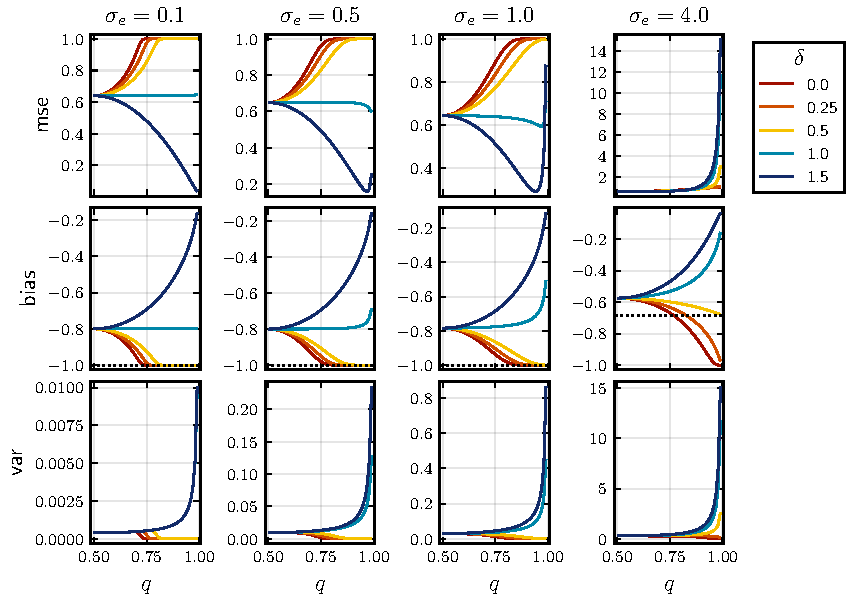
\includegraphics[]{plots/bias-var-onedim.pdf}
  \caption{%
    Bias, variance, and mean-squared error for a one-dimensional lasso problem.
    Note that \(\delta = 0\) corresponds to the case of no scaling, \(\delta = 1/2\) corresponds
    to standardization, and \(\delta = 1\) corresponds to scaling with the variance. The dotted
    lines represent the asymptotic bias of the lasso estimator in the case of \(\delta = 1/2\).
  }
  \label{fig:bias-var-onedim-lasso}
\end{figure}

\subsection{Multiple Predictors}

\begin{figure}[htpb]
  \centering
  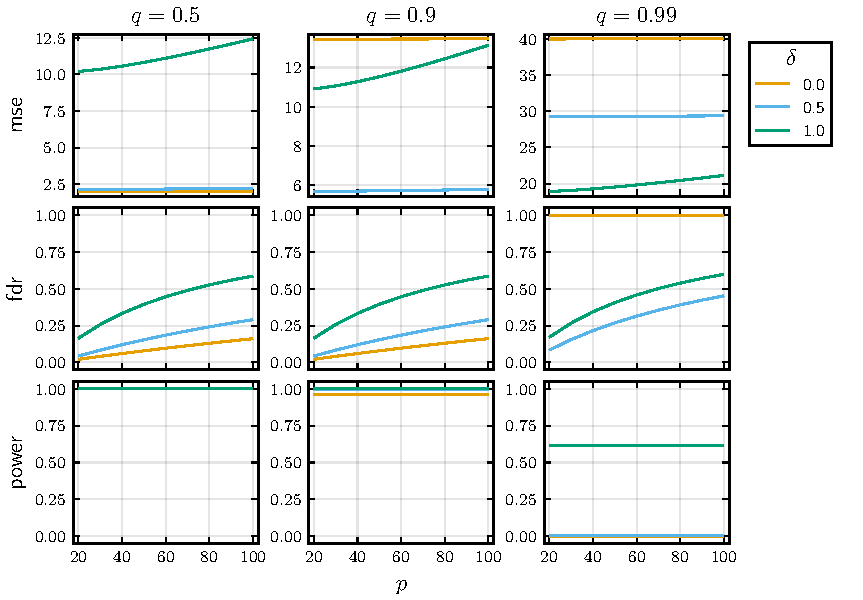
\includegraphics[]{plots/beta-bias-multidim.pdf}
  \caption{%
    Mean-squared-error, false discovery rate (FDR), and power for a lasso problem with
    \(k = 10\) true signals (nonzero \(\beta_j^*\)), varying \(p\), and \(q \in [0.5, 0.9, 0.99]\). The noise level is set at \(\sigma_\varepsilon = 1\).
  }
  \label{fig:mse-fdr-power-multidim}
\end{figure}
